\chapter{Introduction}
\section{Wikimedia and Wikidata}\label{introduction}

The Wikimedia foundation is a non-profit organization whose goal it is to support and encourage free knowledge projects(should i add that they're free of charge and publicly available or is that clear?) such as Wikipedia and Wikidata.

Wikidata was launched in 2012 by the Wikimedia foundation to support other Wikimedia projects (e.g. Wikipedia, Wikisource etc. but also 3rd party projects) by providing a free linked database of structured data. Structured data is is machine readable and is usually stored in a relational database. All data is community-generated and maintained and published under a free license (CC0 1.0). It is inherently multi lingually available and can thus be used across many platforms.

\todo[noline, inline, color=blue!20]{Explaining how it works}

\begin{figure}[h]
	\centering
	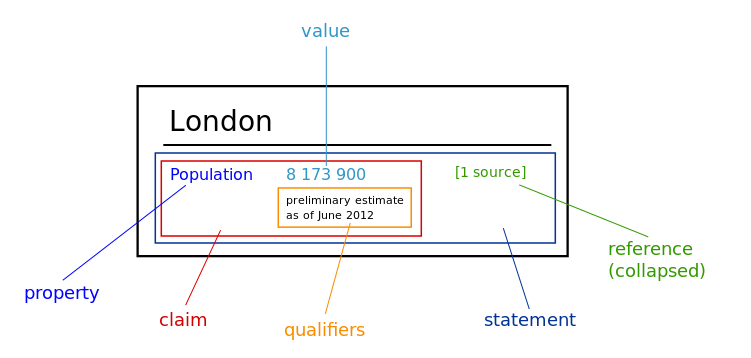
\includegraphics[width=1\textwidth]{Figures/statement.png}
	\caption{\textit{Composition of an Item}: This diagram shows the structure of an \textit{item} in \textit{Wikidata}}
\end{figure}

Most objects in the database consist of items. Items have descriptions and labels which have statements. These statements have properties which hold a value and qualifiers Every item statement of an item should have references.


It is a secondary \todo[fancyline, color=blue!20]{insert this somehow} database because it also stores sources to all objects


\section{Initial Problem Statement}


As of (07.10.15), Wikidata has almost 15 million entries. This broad database is not as heavily utilized as hoped for by the organization and its community. It has been hypothesized that this is most likely caused by a multitude of reasons which possibly include the lack of usability of the data integration and editing functions and their visibility.

Currently the editing process involves being directed away from the client, and after completing the edit, being redirected back to the client. This makes many users uncomfortable because they are leaving their comfort zone which is on their local Wiki. Often one can witness a basic lack of understanding what Wikidata is amongst other Wiki users/editors. 
In Wikidata you can have multiple sets of the same statement with different data backed up by different sources. Wikidata is a platform for free knowledge not for imposing the true knowledge on anyone. Unlike Wikipedia where it must be agreed upon one truth which will be published(not the best word). Thus the habit of editing of Wikipedia editors is one of replacing and not adding which is what is required when editing Wikidata. 
Another problem that most Wikis face is that most communities prefer not to deviate form their own Wiki. It's outsourcing data (in a way) and thus handing over control and responsibility to a certain extent although preferably the loyalty should be to all Wikimedia projects and not separated into the separate Wikis. 
Unfortunately the Wiki communities have had a bad experience when Wiki commons came out. (cite)

To improve the current editing situation a concept is needed that that will ease the editing process for the editors when working from a client such as Wikipedia. (From now on, client will stand for Wikipedia unless otherwise specified). The field of usability yields many methods and tools to approach this problem. In the scope of this thesis many will be tested and used to narrow down the possibilities to an optimal solution. There is no one way to approach a problem like this. 
Another big task will be to keep all communities involved satisfied. The various Wiki communities are know to have (source?) very strong bongs to their respective Wikis and usually don't welcome changes to them. Thus it will be very important to convey a sense of ownership when working with them. It can be assumed that an implementation of any kind will not result in success, which is defined by how frequently the feature is ends up being used, if the community is not going to be involved in the process of development. 

\section{Requirements Analysis}
It must be ensured that vandalism is not being facilitated, which would otherwise consequentially degrade the data quality while still having a low entry barrier.
Another important issue is one of locality. Things that happen locally must also convey that that, as well as things that are happening remotely, otherwise the user can get confused about where the edit is happening. 

It will be important to create a sense of ownership when coming up with a concept because otherwise there is a chance of the community feeling overlooked. (make a section for community?)

The ISO standard 9241-210:2010 (Ergonomics of human-system interaction -- Part 210: Human-centred design for interactive systems), describes what user centered design is in 6 principles:




\clearpage %force page break